\documentclass{standalone}
\usepackage{tikz}
\usetikzlibrary{patterns, positioning}


\begin{document}
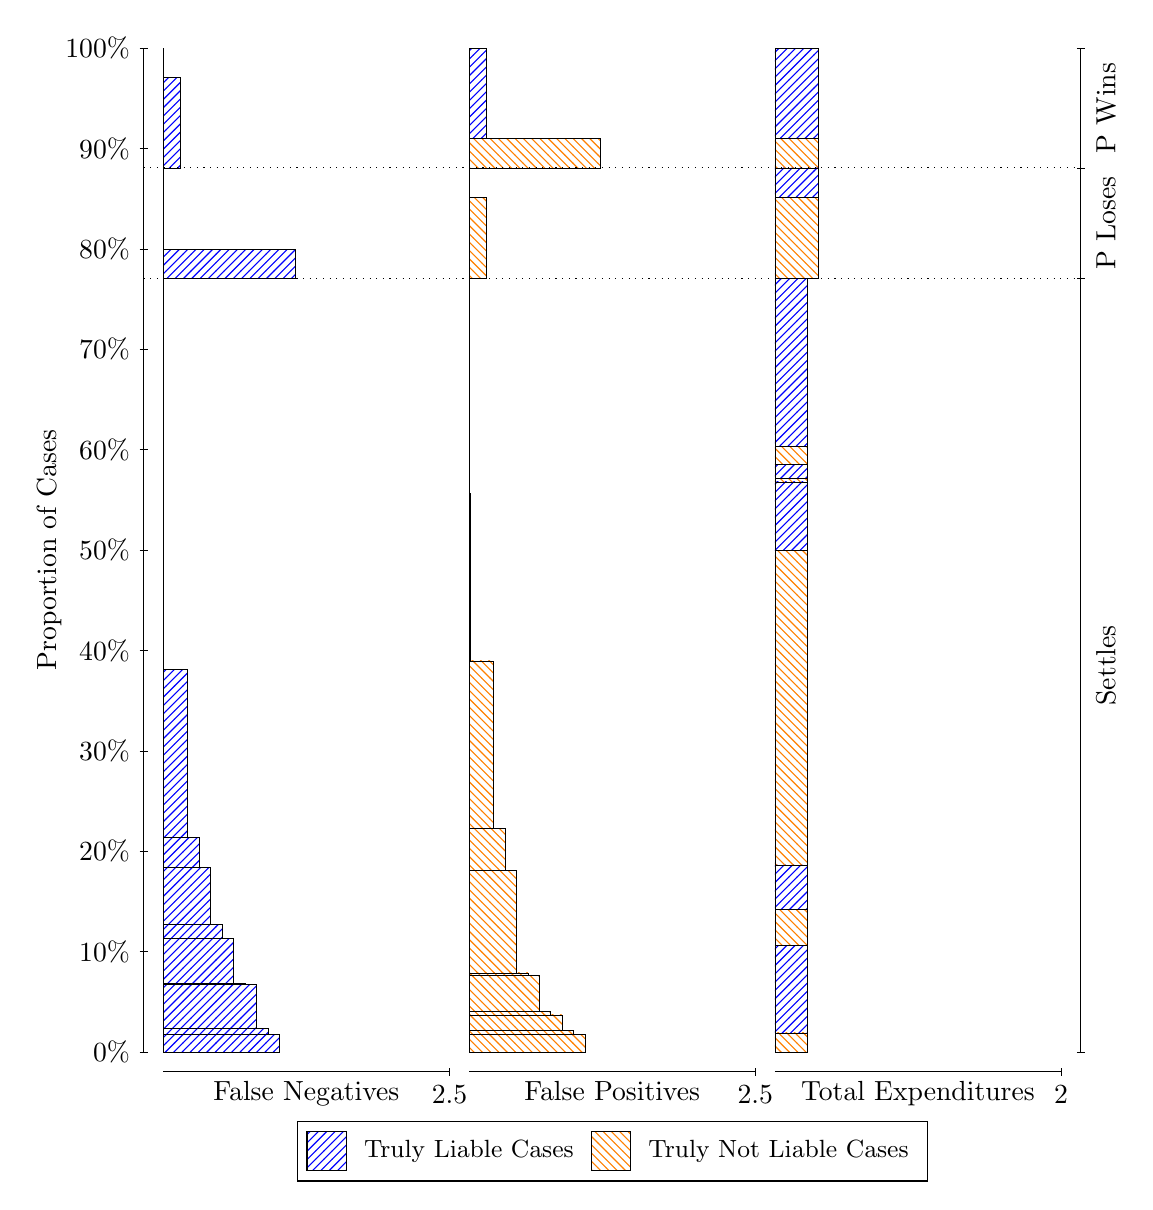
\begin{tikzpicture}
\draw[black, very thin] (1.5,1.75) -- (1.5,14.5);
\node[rotate=90, text=black, anchor=center] at (0.3, 8.125) {Proportion of Cases};
\draw[black, very thin] (1.45,1.75) -- (1.55,1.75);
\node[text=black, anchor=east] at (1.45, 1.75) {0\%};
\draw[black, very thin] (1.45,3.025) -- (1.55,3.025);
\node[text=black, anchor=east] at (1.45, 3.025) {10\%};
\draw[black, very thin] (1.45,4.3) -- (1.55,4.3);
\node[text=black, anchor=east] at (1.45, 4.3) {20\%};
\draw[black, very thin] (1.45,5.575) -- (1.55,5.575);
\node[text=black, anchor=east] at (1.45, 5.575) {30\%};
\draw[black, very thin] (1.45,6.85) -- (1.55,6.85);
\node[text=black, anchor=east] at (1.45, 6.85) {40\%};
\draw[black, very thin] (1.45,8.125) -- (1.55,8.125);
\node[text=black, anchor=east] at (1.45, 8.125) {50\%};
\draw[black, very thin] (1.45,9.4) -- (1.55,9.4);
\node[text=black, anchor=east] at (1.45, 9.4) {60\%};
\draw[black, very thin] (1.45,10.675) -- (1.55,10.675);
\node[text=black, anchor=east] at (1.45, 10.675) {70\%};
\draw[black, very thin] (1.45,11.95) -- (1.55,11.95);
\node[text=black, anchor=east] at (1.45, 11.95) {80\%};
\draw[black, very thin] (1.45,13.225) -- (1.55,13.225);
\node[text=black, anchor=east] at (1.45, 13.225) {90\%};
\draw[black, very thin] (1.45,14.5) -- (1.55,14.5);
\node[text=black, anchor=east] at (1.45, 14.5) {100\%};

\draw[black, very thin] (13.4,1.75) -- (13.4,14.5);
\draw[black, very thin] (13.35,1.75) -- (13.45,1.75);
\node[anchor=west] at (13.35, 1.75) {};
\draw[black, very thin] (13.35,11.57) -- (13.45,11.57);
\node[anchor=west] at (13.35, 11.57) {};
\draw[black, very thin] (13.35,12.979) -- (13.45,12.979);
\node[anchor=west] at (13.35, 12.979) {};
\draw[black, very thin] (13.35,14.5) -- (13.45,14.5);
\node[anchor=west] at (13.35, 14.5) {};

\draw[black, very thin, pattern color=blue, pattern=north east lines] (1.75,1.75) rectangle (3.2215,1.9779);
\draw[black, very thin, pattern color=blue, pattern=north east lines] (1.75,1.9779) rectangle (3.0762,2.0503);
\draw[black, very thin, pattern color=blue, pattern=north east lines] (1.75,2.0503) rectangle (2.9308,2.6087);
\draw[black, very thin, pattern color=blue, pattern=north east lines] (1.75,2.6087) rectangle (2.7855,2.6233);
\draw[black, very thin, pattern color=blue, pattern=north east lines] (1.75,2.6233) rectangle (2.6402,3.1921);
\draw[black, very thin, pattern color=blue, pattern=north east lines] (1.75,3.1921) rectangle (2.4948,3.372);
\draw[black, very thin, pattern color=blue, pattern=north east lines] (1.75,3.372) rectangle (2.3495,4.0951);
\draw[black, very thin, pattern color=blue, pattern=north east lines] (1.75,4.0951) rectangle (2.2042,4.4782);
\draw[black, very thin, pattern color=blue, pattern=north east lines] (1.75,4.4782) rectangle (2.0588,6.604);
\draw[black, very thin, pattern color=orange, pattern=north west lines] (1.75,6.604) rectangle (1.75,11.57);
\draw[black, very thin, pattern color=blue, pattern=north east lines] (1.75,11.57) rectangle (3.4213,11.944);
\draw[black, very thin, pattern color=orange, pattern=north west lines] (1.75,11.944) rectangle (1.75,12.979);
\draw[black, very thin, pattern color=blue, pattern=north east lines] (1.75,12.979) rectangle (1.968,14.125);
\draw[black, very thin, pattern color=orange, pattern=north west lines] (1.75,14.125) rectangle (1.75,14.5);
\draw[black, very thin, pattern color=orange, pattern=north west lines] (5.6333,1.75) rectangle (7.1048,1.9779);
\draw[black, very thin, pattern color=orange, pattern=north west lines] (5.6333,1.9779) rectangle (6.9595,2.0193);
\draw[black, very thin, pattern color=orange, pattern=north west lines] (5.6333,2.0193) rectangle (6.8142,2.2205);
\draw[black, very thin, pattern color=orange, pattern=north west lines] (5.6333,2.2205) rectangle (6.6688,2.2661);
\draw[black, very thin, pattern color=orange, pattern=north west lines] (5.6333,2.2661) rectangle (6.5235,2.7235);
\draw[black, very thin, pattern color=orange, pattern=north west lines] (5.6333,2.7235) rectangle (6.3782,2.7557);
\draw[black, very thin, pattern color=orange, pattern=north west lines] (5.6333,2.7557) rectangle (6.2328,4.0587);
\draw[black, very thin, pattern color=orange, pattern=north west lines] (5.6333,4.0587) rectangle (6.0875,4.5896);
\draw[black, very thin, pattern color=orange, pattern=north west lines] (5.6333,4.5896) rectangle (5.9422,6.7156);
\draw[black, very thin, pattern color=blue, pattern=north east lines] (5.6333,6.7156) rectangle (5.6515,8.8414);
\draw[black, very thin, pattern color=blue, pattern=north east lines] (5.6333,8.8414) rectangle (5.6333,11.57);
\draw[black, very thin, pattern color=orange, pattern=north west lines] (5.6333,11.57) rectangle (5.8513,12.605);
\draw[black, very thin, pattern color=blue, pattern=north east lines] (5.6333,12.605) rectangle (5.6333,12.979);
\draw[black, very thin, pattern color=orange, pattern=north west lines] (5.6333,12.979) rectangle (7.3047,13.353);
\draw[black, very thin, pattern color=blue, pattern=north east lines] (5.6333,13.353) rectangle (5.8513,14.5);
\draw[black, very thin, pattern color=orange, pattern=north west lines] (9.5167,1.75) rectangle (9.9254,1.9927);
\draw[black, very thin, pattern color=blue, pattern=north east lines] (9.5167,1.9927) rectangle (9.9254,3.0988);
\draw[black, very thin, pattern color=orange, pattern=north west lines] (9.5167,3.0988) rectangle (9.9254,3.5563);
\draw[black, very thin, pattern color=blue, pattern=north east lines] (9.5167,3.5563) rectangle (9.9254,4.1251);
\draw[black, very thin, pattern color=orange, pattern=north west lines] (9.5167,4.1251) rectangle (9.9254,8.1171);
\draw[black, very thin, pattern color=blue, pattern=north east lines] (9.5167,8.1171) rectangle (9.9254,8.9904);
\draw[black, very thin, pattern color=orange, pattern=north west lines] (9.5167,8.9904) rectangle (9.9254,9.0359);
\draw[black, very thin, pattern color=blue, pattern=north east lines] (9.5167,9.0359) rectangle (9.9254,9.2159);
\draw[black, very thin, pattern color=orange, pattern=north west lines] (9.5167,9.2159) rectangle (9.9254,9.4437);
\draw[black, very thin, pattern color=blue, pattern=north east lines] (9.5167,9.4437) rectangle (9.9254,11.57);
\draw[black, very thin, pattern color=orange, pattern=north west lines] (9.5167,11.57) rectangle (10.062,12.605);
\draw[black, very thin, pattern color=blue, pattern=north east lines] (9.5167,12.605) rectangle (10.062,12.979);
\draw[black, very thin, pattern color=orange, pattern=north west lines] (9.5167,12.979) rectangle (10.062,13.353);
\draw[black, very thin, pattern color=blue, pattern=north east lines] (9.5167,13.353) rectangle (10.062,14.5);
\draw[black, dotted] (1.5,11.57) -- (13.4,11.57);
\draw[black, dotted] (1.5,12.979) -- (13.4,12.979);
\draw[black, very thin] (1.75,1.5) -- (5.3833,1.5);
\node[text=black, anchor=north] at (3.5667, 1.5) {False Negatives};
\draw[black, very thin] (5.3833,1.45) -- (5.3833,1.55);
\node[text=black, anchor=north] at (5.3833, 1.45) {2.5};

\draw[black, very thin] (5.6333,1.5) -- (9.2667,1.5);
\node[text=black, anchor=north] at (7.45, 1.5) {False Positives};
\draw[black, very thin] (9.2667,1.45) -- (9.2667,1.55);
\node[text=black, anchor=north] at (9.2667, 1.45) {2.5};

\draw[black, very thin] (9.5167,1.5) -- (13.15,1.5);
\node[text=black, anchor=north] at (11.333, 1.5) {Total Expenditures};
\draw[black, very thin] (13.15,1.45) -- (13.15,1.55);
\node[text=black, anchor=north] at (13.15, 1.45) {2};

\node[text=black, centered, rotate=90] at (13.72, 6.6598) {Settles};
\node[text=black, centered, rotate=90] at (13.72, 12.274) {P Loses};
\node[text=black, centered, rotate=90] at (13.72, 13.739) {P Wins};

\draw (7.449999999999999,1.5) node[draw=none] (baseCoordinate) {};
\begin{scope}[align=center]
        \matrix[scale=0.5, draw=black, below=0.5cm of baseCoordinate, nodes={draw}, column sep=0.1cm]{
            \node[rectangle, draw, minimum width=0.5cm, minimum height=0.5cm, pattern color=blue, pattern=north east lines] {}; &
            \node[draw=none, font=\small, text=black] (B) {Truly Liable Cases}; &
            \node[rectangle, draw, minimum width=0.5cm, minimum height=0.5cm, pattern color=orange, pattern=north west lines] {}; &
            \node[draw=none, font=\small, text=black] (B) {Truly Not Liable Cases}; \\
            };
\end{scope}

\end{tikzpicture}
\end{document}